\documentclass[11pt,letterpaper]{article}

\usepackage[margin=1in]{geometry}
\usepackage{times}
\usepackage{setspace}
\usepackage{graphicx}
\usepackage{booktabs}
\usepackage{tabularx}
\usepackage{amsmath,amssymb}
\usepackage{hyperref}
\usepackage{caption}
\usepackage{xcolor}
\usepackage{enumitem}
\usepackage[T1]{fontenc}
\usepackage[utf8]{inputenc}

\hypersetup{colorlinks=true,linkcolor=black,citecolor=black,urlcolor=blue}
\graphicspath{{figures/}}
\onehalfspacing
\setlength{\parskip}{0.4em}

\title{\textbf{Reconstructing Canadian Housing Hardship, 2011--2021:\\
Household Residual Income versus the Non-Shelter Market Basket Measure}}
\author{High School Research Paper\\[0.4em]
\large Draft Version 4.0}
\date{17 October 2026}

\begin{document}
\maketitle

\begin{abstract}
\noindent\textbf{Background.}
Drafts 1--3 treated hierarchical Census person-records as if they were households, used a single-adult leftover line, and dropped 2016 because only 9.4\% of rows survived a renter-only cleaner. Those choices do not match Statistics Canada file structure or the CMHC housing-hardship definition.

\noindent\textbf{Objective.}
Rebuild the analysis from the original PUMFs and official data dictionaries. Measure leftover income at the household, apply survey weights, and compare residual income with the non-shelter Market Basket Measure.

\noindent\textbf{Methods.}
We collapse four hierarchical PUMFs to one row per household. After-tax income is the sum of person \texttt{TOTINC\_AT} after official missing codes. Shelter is maintainer \texttt{OMP}/\texttt{GROSRT} (2006, 2011) or \texttt{SHELCO} (2016, 2021). Hardship is residual income below the Table~11-10-0066 non-shelter MBM scaled by $\sqrt{n}/2$. Rates use household \texttt{WEIGHT}. The 2006 all-household wave is not comparable (shelter code 8888). These are reconstructed research rates, not official CMHC statistics.

\noindent\textbf{Results.}
Among weighted households, reconstructed hardship is 18.2\% in the 2011 NHS, 17.3\% in 2016, and 14.9\% in 2021. Renters remain about three times as likely as owners to be in hardship (27.6\% versus 8.8\% in 2021). Median after-tax income matches published Census medians to within 1.4\% for 2011--2021. The 2021 core-need flag on the same file is 10.12\% versus the published 10.1\%.

\noindent\textbf{Conclusions.}
Once the unit, weights, file identity and MBM definition are repaired, the Draft~3 story of a stable $\sim$38\% crisis does not hold. Leftover-income pressure is still high for renters and one-person households, but the comparable household series declines modestly from 2011 to 2021. Official CMHC rates would be lower still.

\medskip
\noindent\textit{Keywords:} housing affordability; residual income; Market Basket Measure; Census PUMF; CMHC; Canada
\end{abstract}

\tableofcontents
\newpage

\section{Introduction}
\label{sec:intro}

The usual school rule says housing is affordable if it costs less than 30\% of income.
That rule can hide a household that spends 25\% on rent and still cannot buy food and bus fare.
Canada Mortgage and Housing Corporation (CMHC) therefore also asks a leftover-income question: after housing is paid, is there enough money left for the non-housing part of Canada's official poverty line, the Market Basket Measure (MBM) \cite{cmhc2020,statcan2021mbm}?

Drafts 1--3 of this paper tried to answer that question with Census Public Use Microdata Files (PUMF) for 2006, 2011 and 2021.
They reported hardship near 38\%, 34\% and 38\%.
Those numbers cannot be used.
The local files were mislabeled, person income was treated as household income, owners were dropped on pre-2016 files, survey weights were ignored, and the MBM line was a single-adult leftover, not the official non-shelter, size-adjusted basket.

Draft 4.0 starts over from the original Statistics Canada files and official tables.
It asks three questions that can actually be answered with these PUMFs:

\begin{enumerate}[leftmargin=1.6em]
  \item After households, weights and the non-shelter MBM are constructed correctly, how does reconstructed hardship change from 2011 to 2021?
  \item Can 2016 be used, and can 2006?
  \item How far are the reconstructed rates from published Statistics Canada and CMHC statistics, and why?
\end{enumerate}

\section{Methods}
\label{sec:methods}

\subsection{Files and identity}

Hierarchical PUMFs are person records nested in households (\texttt{HH\_ID}).
Local filenames do not match census years.

\begin{center}
\small
\begin{tabular}{llllr}
\toprule
Local file & Official file & Catalogue & Instrument & Households \\
\midrule
\texttt{census\_2006.csv} & 2006 Census hierarchical & 95M0029X & Long form 2B & 124,358 \\
\texttt{census\_2006\_pumf.csv} & 2011 NHS hierarchical & 99M0002X & Voluntary NHS & 133,192 \\
\texttt{census\_2011\_nhs.csv} & 2016 Census hierarchical & 98M0002X & Census 2A-L & 140,720 \\
\texttt{census\_2021\_full.csv} & 2021 Census hierarchical & 98M0002X & Census 2A-L & 149,789 \\
\bottomrule
\end{tabular}
\end{center}

\texttt{census\_2016\_pumf.csv} is a duplicate of the 2006 file and is not used.
Income refers to the previous calendar year (2005, 2010, 2015, 2020).
2011 is a voluntary survey, not a Census long form \cite{statcan2011nhs,statcan2016pumf,statcan2022pumf}.

\subsection{Household construction}

The analytic unit is the household.
After-tax household income is the sum of person \texttt{TOTINC\_AT} after official not-available and not-applicable codes (\texttt{8888888}/\texttt{9999999}; 2011 uses six-digit \texttt{888888}/\texttt{999999}).
Monthly shelter is the primary maintainer's value (\texttt{PRIHM==1}): \texttt{OMP} if owned and \texttt{GROSRT} if rented in 2006/2011; \texttt{SHELCO} in 2016/2021 \cite{statcan2006pumf}.
Shelter is never summed across persons.
The household weight is one copy of \texttt{WEIGHT}.
Person weights are not added.

A household enters the analytic sample if tenure is owner or renter, after-tax income is positive, and monthly shelter is present and in $(0, 10000)$.
Sample $n$ and estimated population $N$ are reported separately.

\subsection{Why 2006 kept 23.4\% and 2016 kept 9.4\% in Draft 3}

Those rates came from a person-level cleaner that picked the last matching shelter column.
On 2006 and 2011 files the last match is \texttt{GROSRT}, so owners coded 9999 drop.
The file labelled 2016 on disk is actually 2006, so the 9.4\% figure is 2006 renters.
The file labelled 2011 is actually 2016, so the 23.4\% figure is the 2011 NHS renters.
After household reconstruction, 2016 retains 99.4\% of households.
2006 retains 42.4\%, because confidentiality code 8888 suppresses shelter for most multi-person households.
The 2006 all-household sample has mean size 1.45 versus about 2.4 later.
It is not in the primary series.
A one-person 2006--2021 cut (95\%+ shelter coverage each wave) is kept as robustness.

\subsection{Reconstructed housing hardship}

CMHC's housing-hardship concept compares leftover income with the \textbf{non-shelter} MBM---food, clothing, transportation and other necessities---not the full poverty line, which already includes shelter \cite{cmhc2020}.
The official MBM is built for two adults and two children and scaled by $\sqrt{n}/2$ \cite{statcan2021mbm}.

\begin{align}
\text{Annual shelter} &= 12 \times \text{monthly shelter} \\
\text{Residual income} &= \text{after-tax household income} - \text{annual shelter} \\
\text{Threshold} &= \text{non-shelter MBM}_{n=4} \times \sqrt{n}/2 \\
\text{Hardship} &= 1 \text{ if residual income} < \text{threshold}
\end{align}

Non-shelter MBM is the unweighted mean of Table 11-10-0066-01 regions, current dollars, contemporaneous official base (2008-base in 2010 and 2015; 2018-base in 2020).
Rates use income-year dollars against same-year MBM dollars.
Medians in figures are converted to 2021 CAD with Table 18-10-0005 (Canada All-items: 2010 = 116.5, 2015 = 126.6, 2020 = 137.0, 2021 = 141.6).

This is \emph{not} an official CMHC rate.
Official CMHC also uses MBM disposable income, about 50 geographic cells, and extra universe rules (negative residual dropped; some high-income and investment-income households cannot be in hardship).
Those rules appear only in the sensitivity table.

\subsection{Validation}

We compare (i)~weighted household counts with published private-household totals, (ii)~median after-tax income with Census medians in 2020-constant dollars, (iii)~before-tax STIR $30$--$99\%$ with official unaffordable-housing rates, and (iv)~2021 \texttt{HCORENEED\_IND} with published core housing need \cite{statcan2022daily}.

\section{Results}
\label{sec:results}

\subsection{Sample}

\begin{table}[ht]
\centering
\caption{Sample flow. Analytic $n$ is households with owner/renter tenure, positive after-tax income, and usable shelter.}
\label{tab:flow}
\small
\begin{tabular}{lrrrr}
\toprule
 & 2006 & 2011 NHS & 2016 & 2021 \\
\midrule
Person records in file & 309,841 & 333,008 & 343,330 & 361,915 \\
Households in file & 124,358 & 133,192 & 140,720 & 149,789 \\
Analytic households $n$ & 52,785 & 130,242 & 139,869 & 148,085 \\
Estimated households $N$ & 5.28M & 13.02M & 14.04M & 14.86M \\
Retention of file households & 42.4\% & 97.8\% & 99.4\% & 98.9\% \\
In primary series & No & Yes & Yes & Yes \\
\bottomrule
\end{tabular}
\end{table}

\subsection{Primary household series, 2011--2021}

\begin{table}[ht]
\centering
\caption{Weighted household estimates. Dollars are 2021 CAD (Table 18-10-0005). Hardship is residual income below the size-adjusted non-shelter MBM. Not official CMHC rates.}
\label{tab:primary}
\small
\begin{tabular}{lrrr}
\toprule
 & 2011 NHS & 2016 & 2021 \\
\midrule
Median after-tax income & \$65,634 & \$69,346 & \$76,485 \\
Median monthly shelter & \$1,094 & \$1,118 & \$1,240 \\
After-tax STIR $>$ 30\% & 29.6\% & 28.9\% & 25.9\% \\
Reconstructed hardship & 18.2\% & 17.3\% & 14.9\% \\
\quad Owners & 10.8\% & 9.4\% & 8.8\% \\
\quad Renters & 34.4\% & 34.2\% & 27.6\% \\
\quad One-person & 32.4\% & 32.2\% & 30.3\% \\
Approximate SE (hardship) & 0.28 pp & 0.42 pp & 0.11 pp \\
\bottomrule
\end{tabular}
\end{table}

Reconstructed hardship falls 3.3~percentage points from 2011 to 2021 (Figure~\ref{fig:national}).
Real median income rises 16.5\%; real median shelter rises 13.4\% (Figure~\ref{fig:index}).
The larger improvement is 2016--2021 (hardship $-2.4$~pp), which includes COVID-19 transfers in 2020 income (Figure~\ref{fig:periods}).
Renters remain far above owners in every wave (Figure~\ref{fig:tenure}).

One-person hardship, the only 2006--2021 cut that does not mix suppressed and unsuppressed shelter, is 28.8\% (2006), 32.4\% (2011), 32.2\% (2016) and 30.3\% (2021).
That series rises after 2006 and eases only slightly by 2021 (Figure~\ref{fig:dash}).

\begin{figure}[ht]
\centering
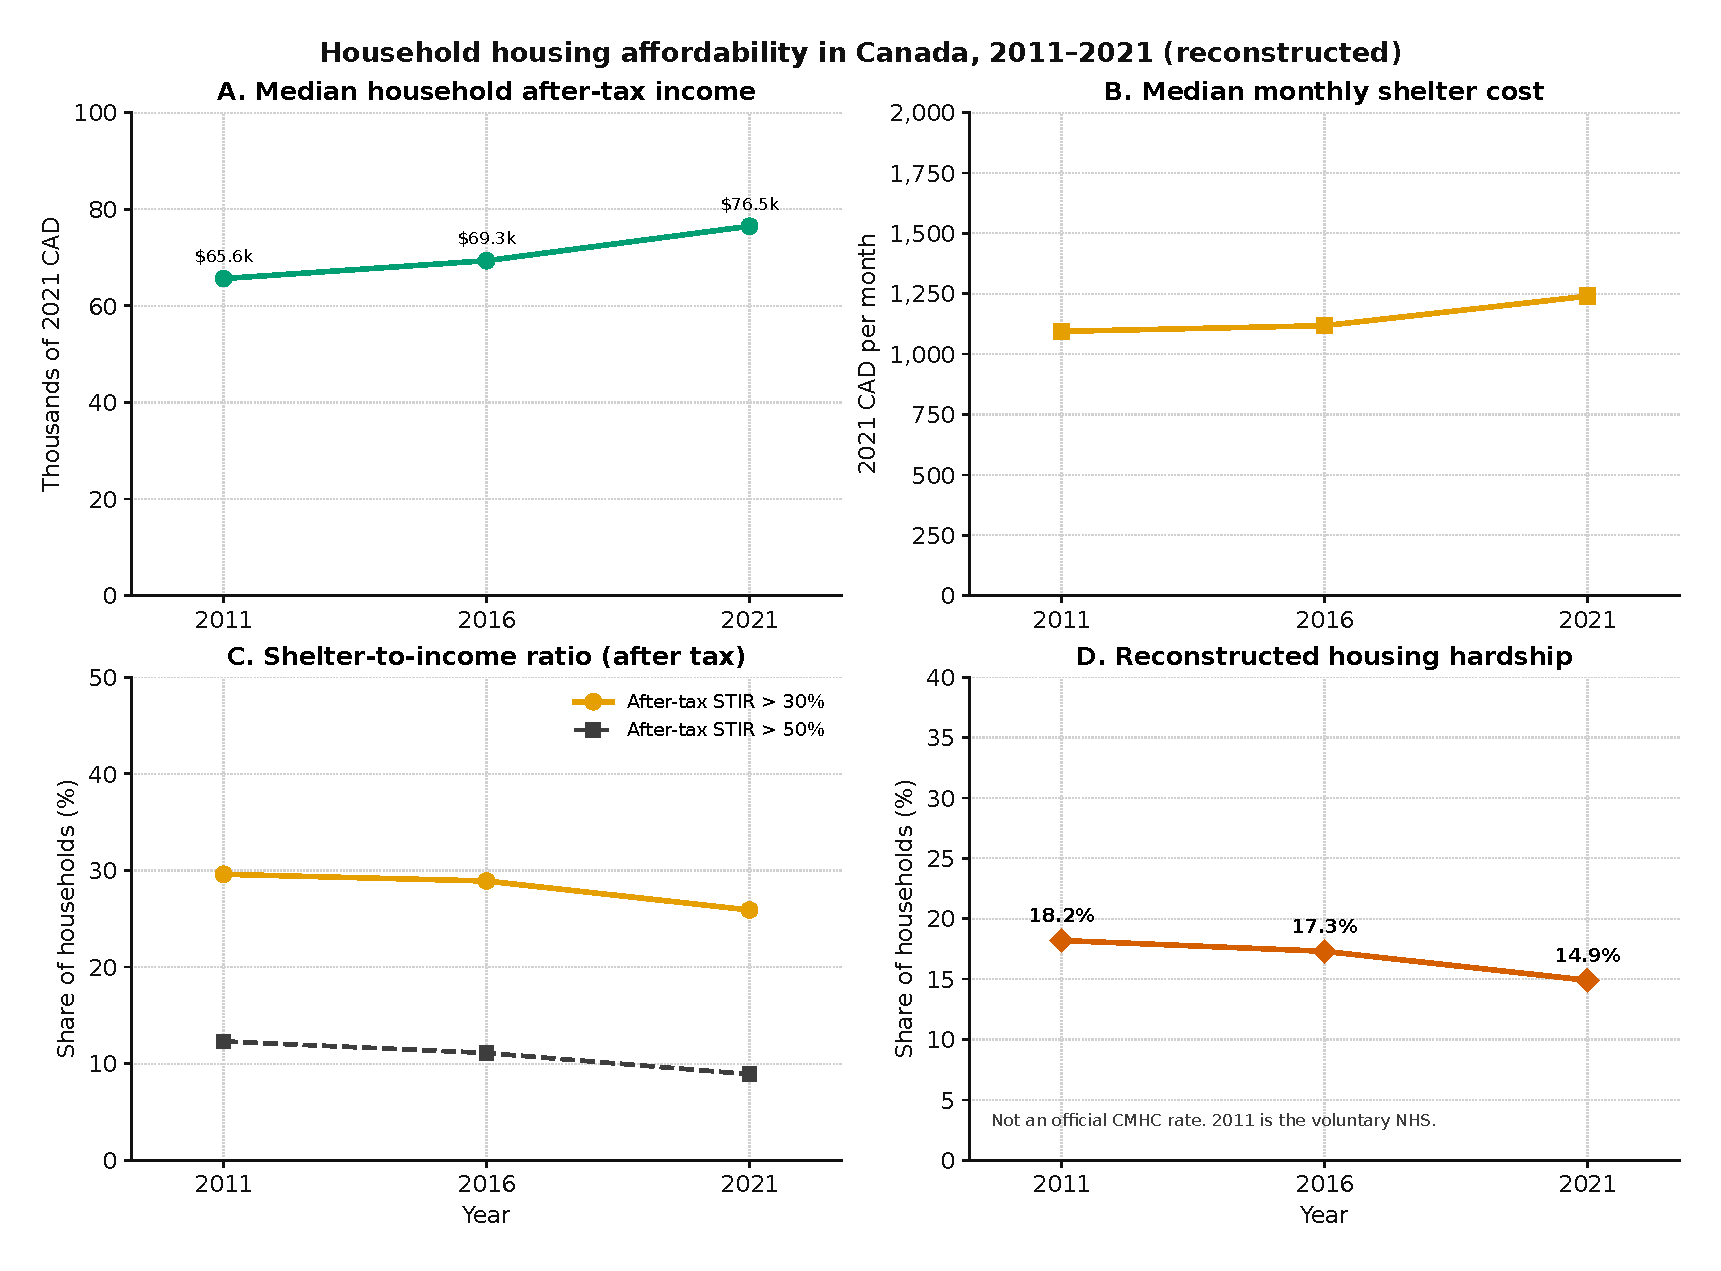
\includegraphics[width=\textwidth]{fig01_national_trends.pdf}
\caption{Weighted household income, shelter, after-tax STIR and reconstructed hardship, 2011--2021. 2011 is the voluntary NHS. Rates are not official CMHC housing-hardship statistics.}
\label{fig:national}
\end{figure}

\begin{figure}[ht]
\centering
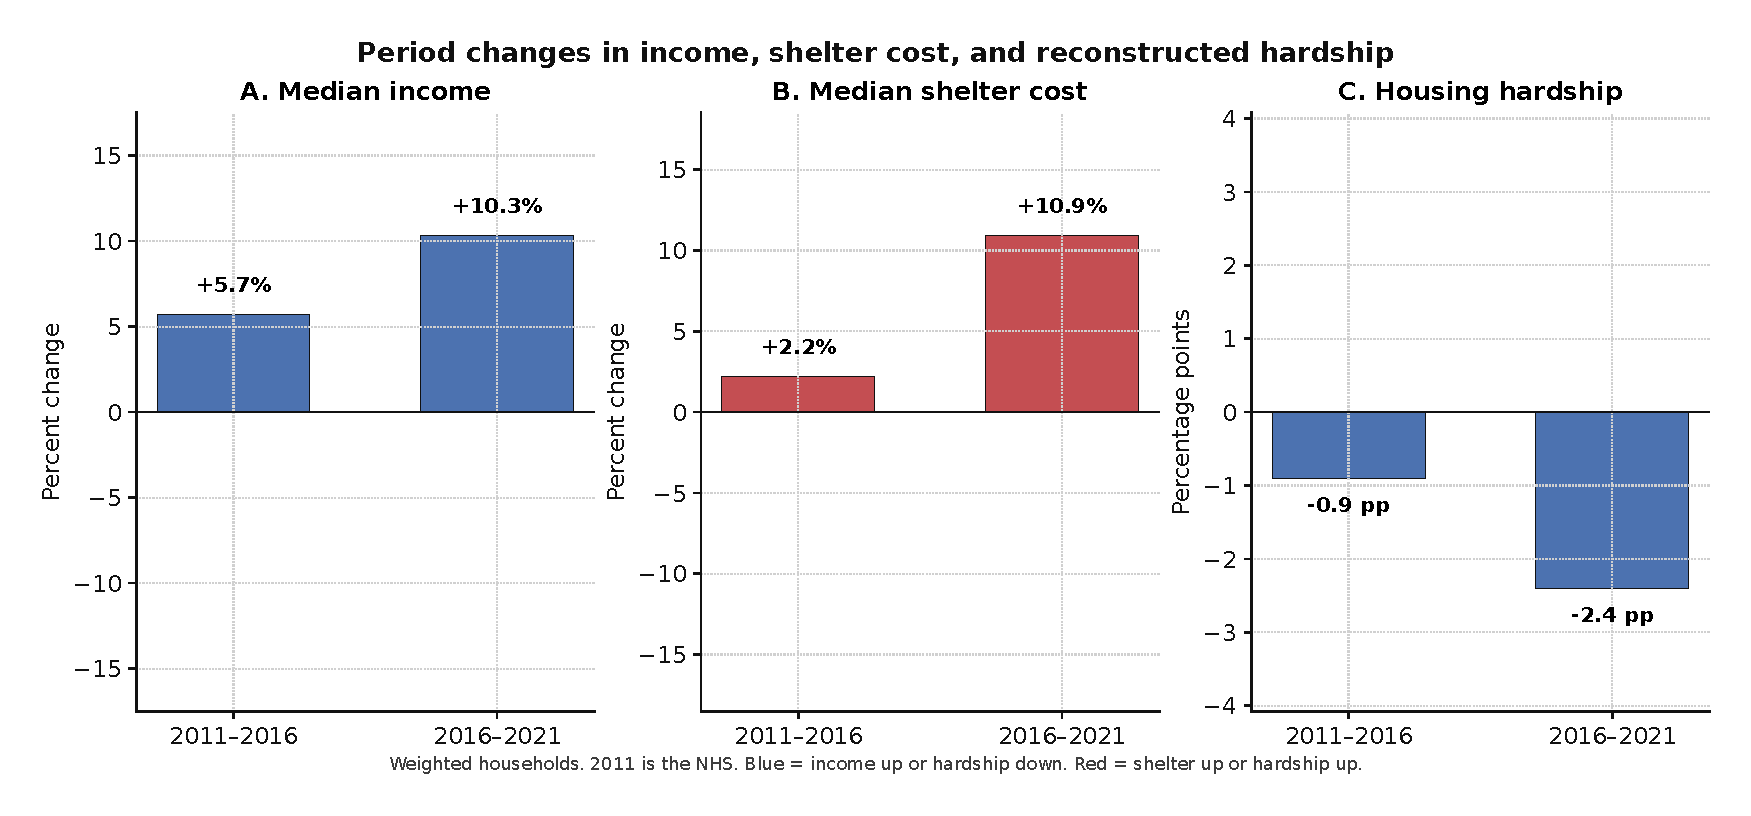
\includegraphics[width=\textwidth]{fig02_period_comparison.pdf}
\caption{Period changes. Income and shelter are percent changes in 2021 CAD medians. Hardship is percentage points.}
\label{fig:periods}
\end{figure}

\begin{figure}[ht]
\centering
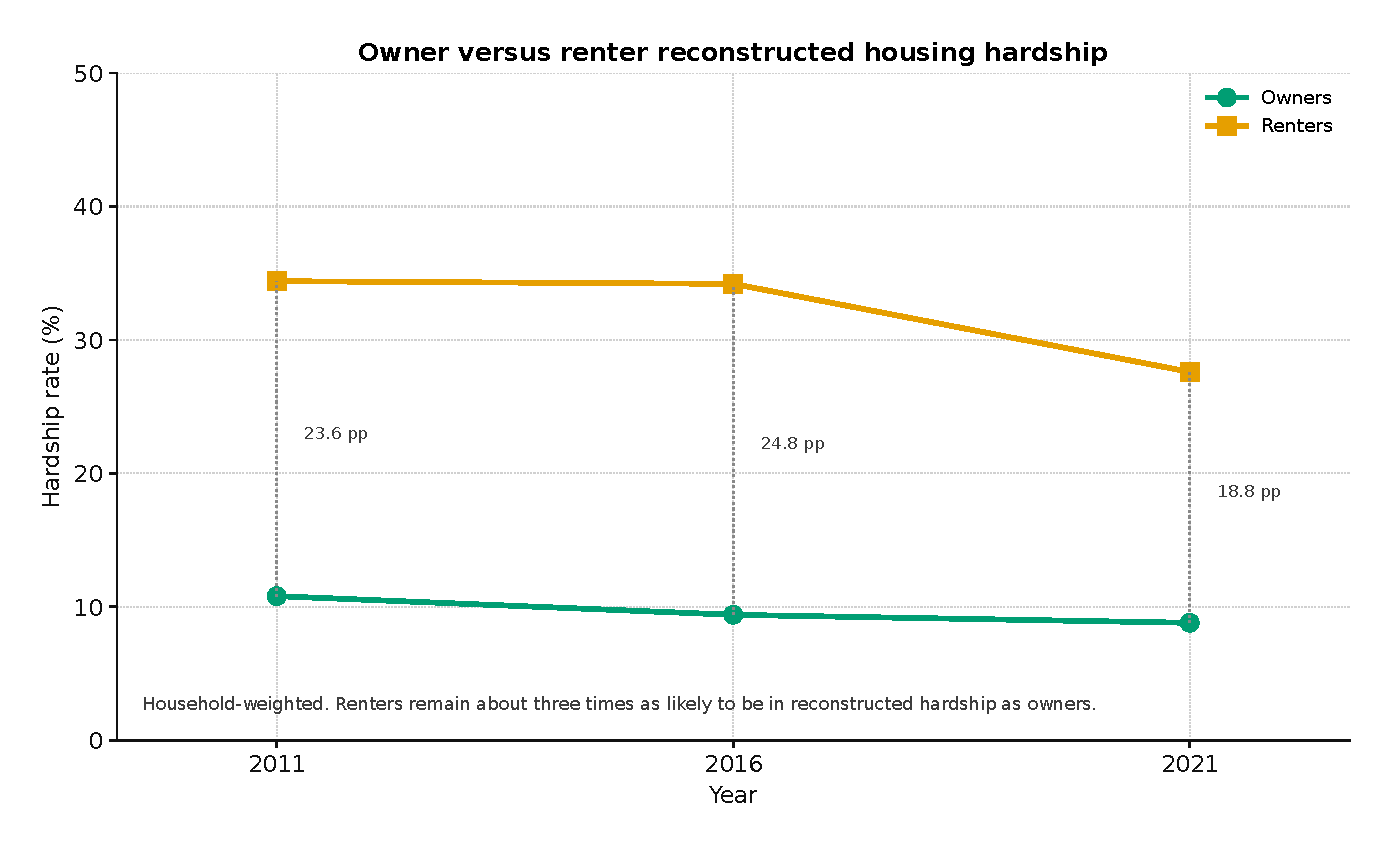
\includegraphics[width=0.85\textwidth]{fig03_tenure_divergence.pdf}
\caption{Owner and renter reconstructed hardship. The gap is 23.6~pp in 2011 and 18.8~pp in 2021.}
\label{fig:tenure}
\end{figure}

\begin{figure}[ht]
\centering
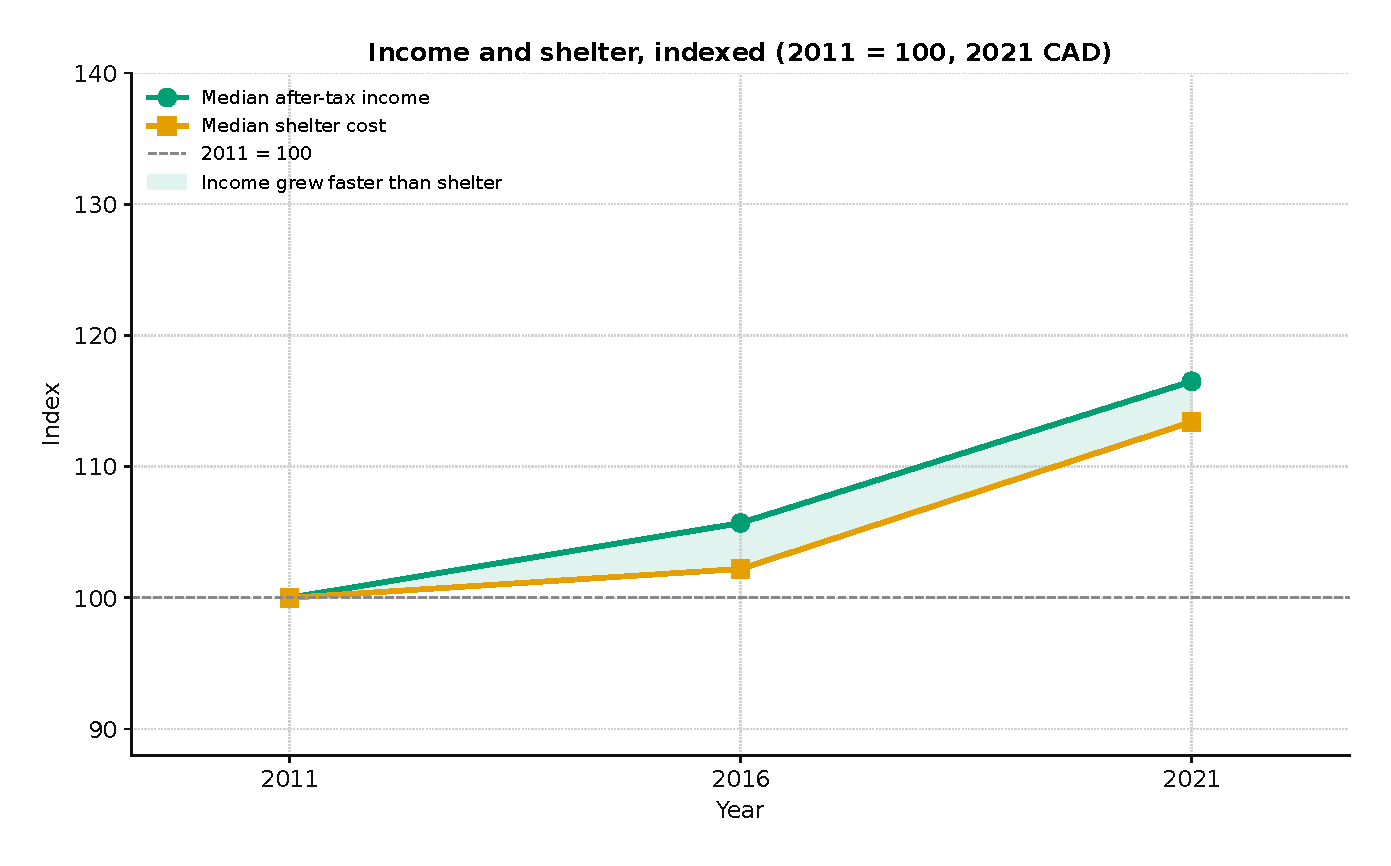
\includegraphics[width=0.85\textwidth]{fig04_income_shelter_index.pdf}
\caption{Median after-tax income and monthly shelter indexed to 2011 $= 100$ (2021 CAD).}
\label{fig:index}
\end{figure}

\begin{figure}[ht]
\centering
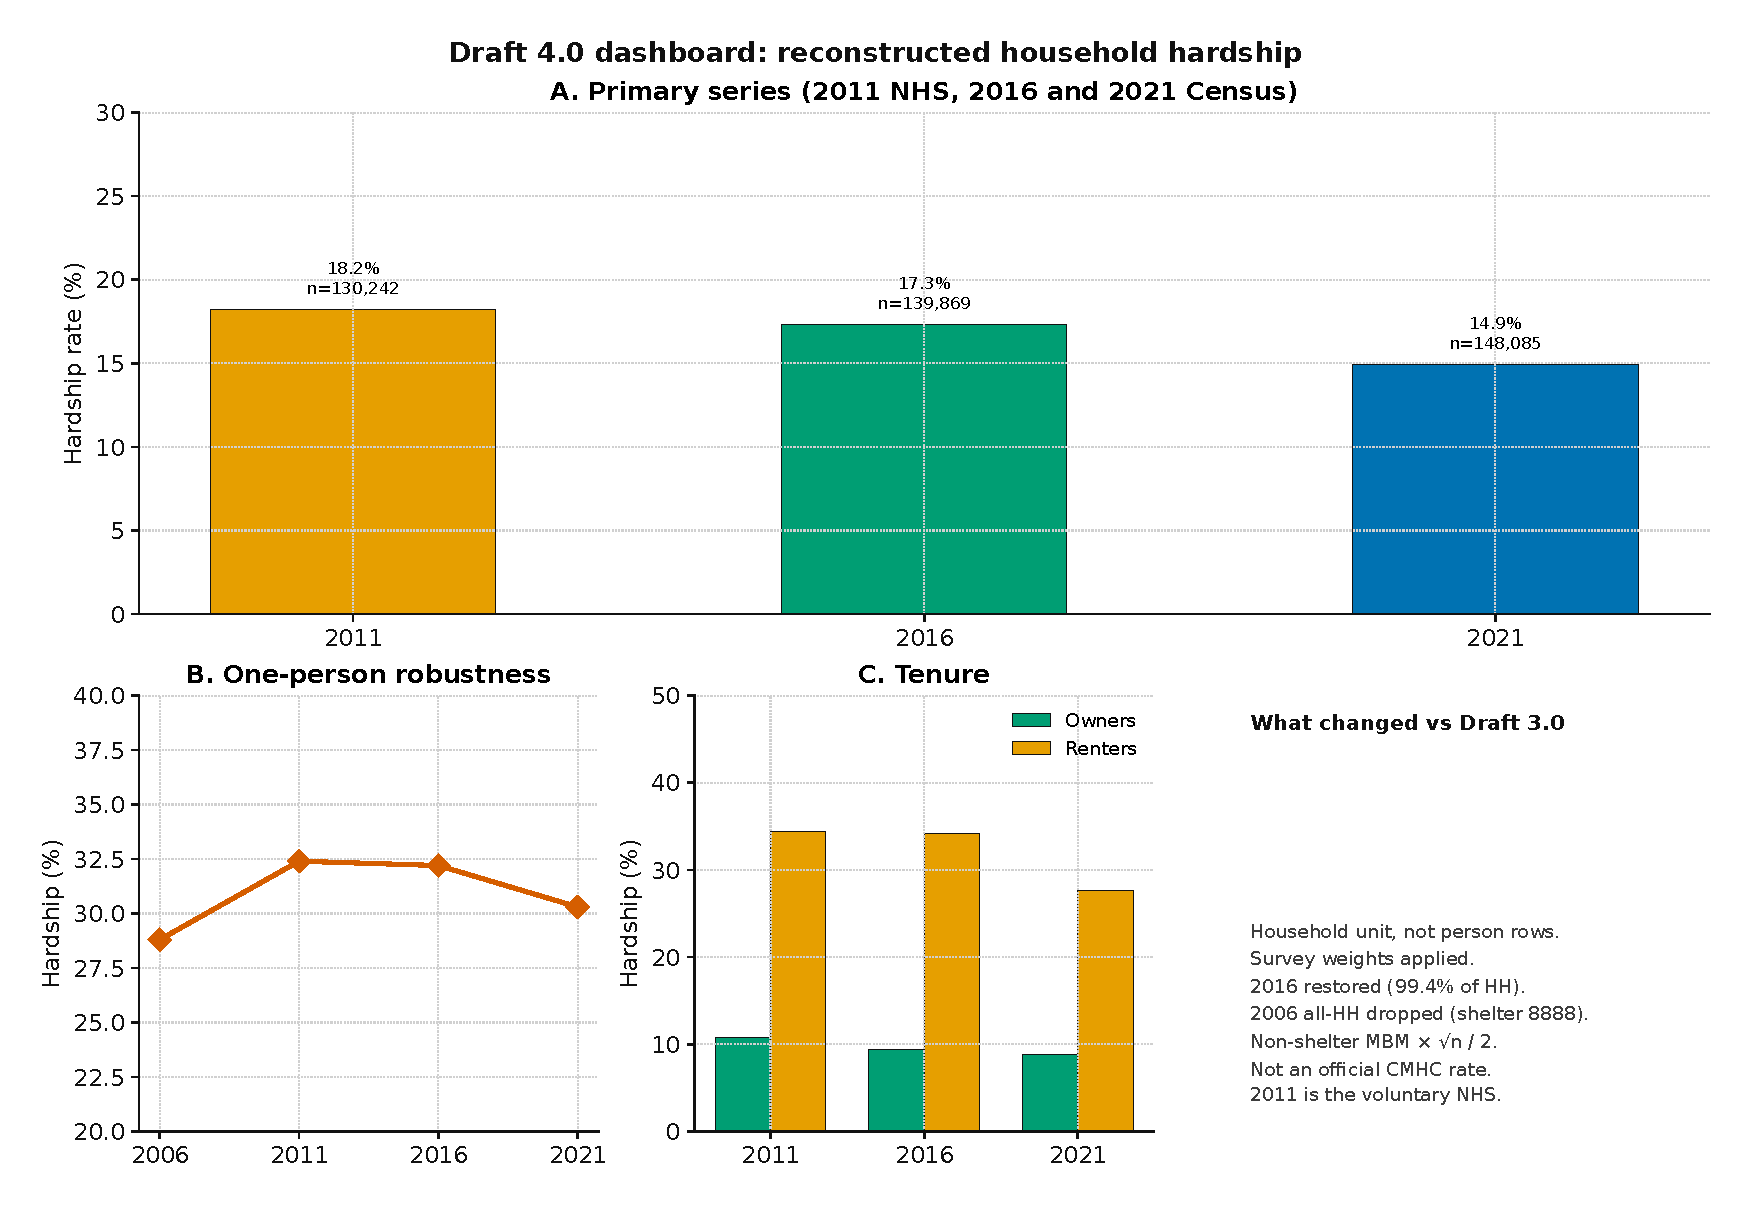
\includegraphics[width=\textwidth]{fig05_summary_dashboard.pdf}
\caption{Primary 2011--2021 series, one-person 2006--2021 robustness, and tenure split.}
\label{fig:dash}
\end{figure}

\subsection{Validation}

Weighted household counts in the four files recover published private-household totals to within 0.4\%.
Median after-tax income in 2020-constant dollars is $\$63{,}502$ versus published $\$63{,}600$ (2011), $\$67{,}093$ versus $\$66{,}500$ (2016), and $\$74{,}000$ versus $\$73{,}000$ (2021).
The 2006 analytic median fails ($-36\%$) because the valid sample is one-person-heavy---further evidence that 2006 all-household hardship must not be plotted with later waves.

Before-tax STIR $30$--$99\%$ is 21.5\% in 2016 and 19.5\% in 2021, against official unaffordable-housing rates of 24.1\% and 20.9\%.
The direction matches; the 1--3~pp gap is consistent with incomplete farm/reserve exclusions and PUMF rounding.
The 2021 \texttt{HCORENEED\_IND} flag is 10.12\% versus published core housing need of 10.1\%.

CMHC's Canadian Income Survey figure of about 9\% hardship in 2017 is \emph{not} a failed replication.
CIS uses MBM disposable income and a tighter universe.
Dropping negative residual income alone moves our 2016 rate from 17.3\% to 14.4\%.
We do not have a recovered official 2021 Census CMHC hardship percentage.

\subsection{Sensitivity}

Using the full MBM as the leftover line---the conceptual error of counting shelter twice---raises hardship by 8--12~points (26.5\% / 25.5\% / 26.6\%).
A single-adult non-shelter line (no size scaling) lowers it by about 3~points.
A CMA/PR geography approximation barely moves 2011 and 2016 and lowers 2021 by 3.1~points.
Weighting barely moves 2016 and 2021 (near self-weighting 1\% samples).
Tenure composition moves the rate more than weighting: renters 34.4\% / 34.2\% / 27.6\% versus owners 10.8\% / 9.4\% / 8.8\%.

\section{Discussion}
\label{sec:discussion}

\subsection{What Draft 3.0 got wrong}

Draft 3.0's 38.0\% / 33.9\% / 37.9\% series was 2011 NHS renters, 2016 persons, and 2021 persons, unweighted, with person income and a simplified leftover line.
It looked like a stable national crisis.
The repaired household series is lower, declines from 2011 to 2021, and still shows a large renter gap.
Both things can be taught: leftover income is a better \emph{question} than the 30\% rule, and the \emph{answer} depends on doing the household arithmetic that Statistics Canada documents.

\subsection{What the repaired series can and cannot say}

It can say that, on these PUMFs, size-adjusted leftover-income hardship among owner and renter households is nearer the teens than the high thirties, and that 2021 is lower than 2011.
It can say 2016 is usable.
It can say 2006 all-household results are not comparable.
It cannot say ``CMHC's official hardship rate is 14.9\% in 2021.''
It cannot treat 2011 as a Census long form.
Part of the 2016--2021 decline may be the 2018-base MBM revision and 2020 emergency benefits, not a permanent easing of housing costs.

\subsection{Limitations}

\begin{enumerate}[leftmargin=1.6em]
  \item PUMF geography is not the official 50-region MBM map.
  \item \texttt{TOTINC\_AT} is not MBM disposable income.
  \item Farm, band and reserve households cannot be fully excluded.
  \item Replicate-weight standard errors use a generic bootstrap formula.
  \item 2006 multi-person shelter is suppressed; 2001 after-tax income does not exist on 95M0020X.
  \item The 2024 CMHC Census hardship update was not recovered.
\end{enumerate}

\section{Conclusion}
\label{sec:conclusion}

After the files are identified, households are collapsed, weights are applied, and leftover income is compared with the non-shelter MBM:

\begin{enumerate}[leftmargin=1.6em]
  \item Reconstructed hardship is 18.2\% (2011 NHS), 17.3\% (2016) and 14.9\% (2021).
  \item 2016 belongs in the series (99.4\% household retention). 2006 all-household results do not.
  \item Renters remain about three times as likely as owners to have too little leftover income.
  \item Household income construction validates against published Census medians for 2011--2021. The 2021 core-need flag matches 10.1\%.
  \item Draft 3.0's $\sim$38\% figures measured a different unit, a different shelter variable and, in two waves, a different year.
\end{enumerate}

The leftover-income question is still the right question.
The Draft~3 numbers were not the right answer.

\begin{thebibliography}{9}

\bibitem{cmhc2020}
Canada Mortgage and Housing Corporation.
\newblock \emph{Introducing the Housing Hardship Concept}.
\newblock Research Insight, January 2020.

\bibitem{statcan2006pumf}
Statistics Canada.
\newblock \emph{2006 Census PUMF Hierarchical File: Documentation and User Guide}.
\newblock Catalogue no.~95M0029XVB.

\bibitem{statcan2011nhs}
Statistics Canada.
\newblock \emph{2011 National Household Survey PUMF Hierarchical File}.
\newblock Catalogue no.~99M0002X.

\bibitem{statcan2016pumf}
Statistics Canada.
\newblock ``2016 Census of Population Public Use Microdata File, Hierarchical File,'' \emph{The Daily}, 18 June 2019.
\newblock Catalogue no.~98M0002X.

\bibitem{statcan2022pumf}
Statistics Canada.
\newblock \emph{Census 2021 Public Use Microdata File (PUMF): Hierarchical File}.
\newblock Catalogue no.~98M0002X, 2022.

\bibitem{statcan2021mbm}
Statistics Canada.
\newblock Table 11-10-0066-01, Market Basket Measure thresholds for the reference family by region, component and base year.
\newblock DOI: 10.25318/1110006601-eng.

\bibitem{statcan2022daily}
Statistics Canada.
\newblock ``To buy or to rent,'' \emph{The Daily}, 21 September 2022.

\bibitem{statcan_cpi}
Statistics Canada.
\newblock Table 18-10-0005-01, Consumer Price Index, annual average, not seasonally adjusted.
\newblock DOI: 10.25318/1810000501-eng.

\end{thebibliography}

\appendix
\section{How to reproduce}
\label{app:repro}

\begin{verbatim}
python3 papers/paper1_draft4/reconstruct_four_wave.py
python3 papers/paper1_draft4/generate_figures_tables.py
cd papers/paper1_draft4
pdflatex paper1_draft4.tex
pdflatex paper1_draft4.tex
\end{verbatim}

Draft 3.0 remains in \texttt{papers/paper1\_highschool/} and is not overwritten.
Original person-level JSON remains at \texttt{results/four\_wave\_temporal\_results.json}.

\end{document}
